\section{Background}
\subsection{Diffusion LLMs}

\begin{figure*}[t!]
    \centering
    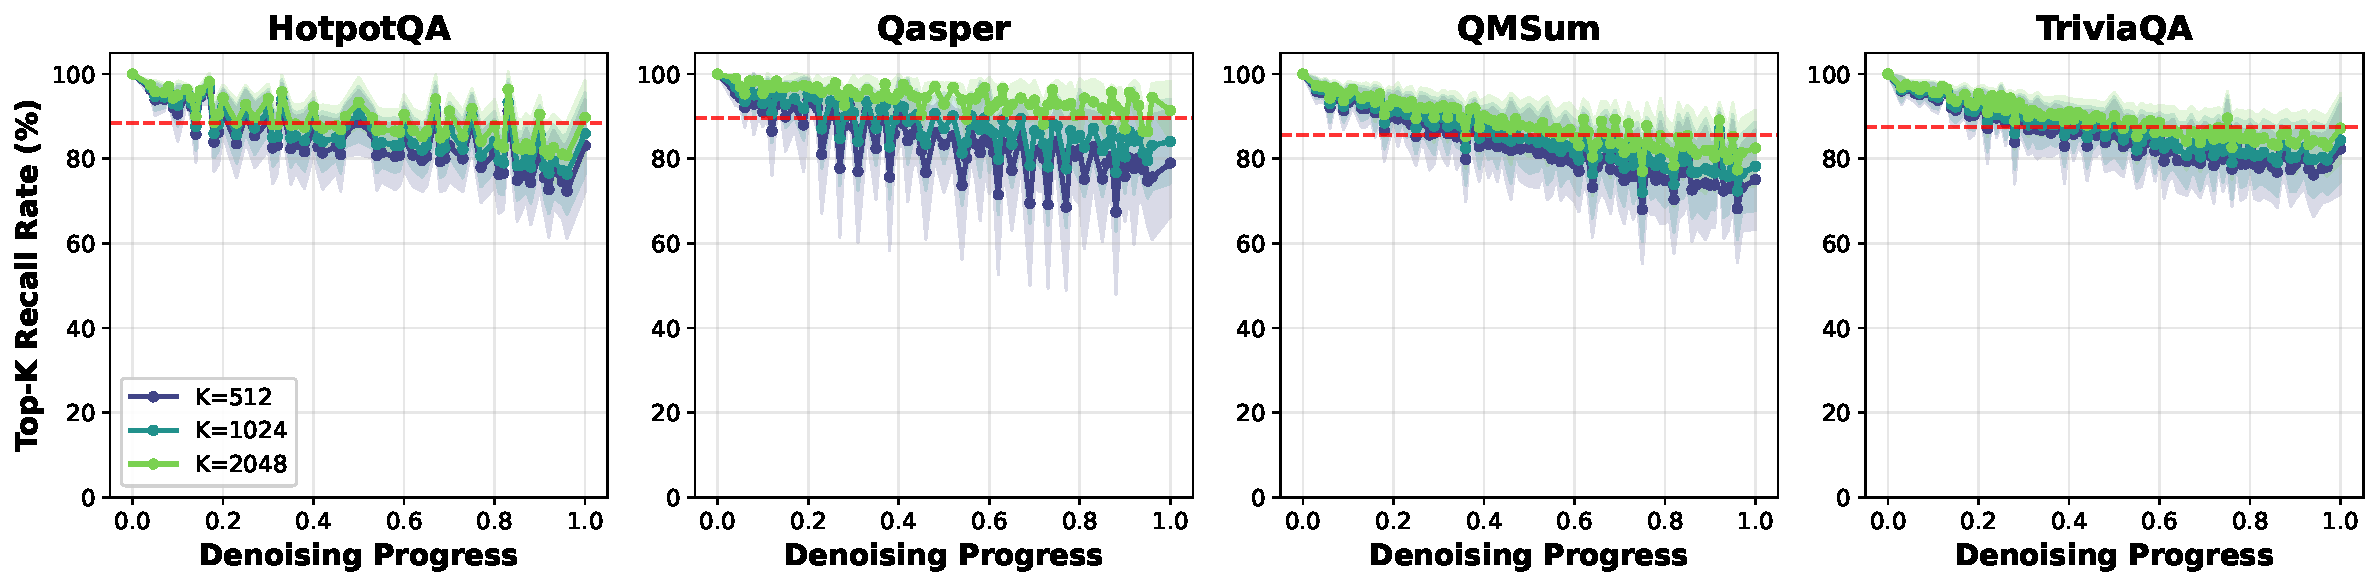
\includegraphics[width=\textwidth]{figures/fig1_mage_consistency_1x4.pdf}
    \caption{Top-K recall rate across denoising steps on LongBench tasks (0: All-\mask block, 1: fully decoded block). The top-K indices selected from the All-\mask block maintain 84--90\% recall throughout denoising.}
    \label{fig:topk_consistency}
\end{figure*}



Diffusion LLMs have emerged as a new paradigm for language generation, breaking the left-to-right sequential dependency of autoregressive (AR) models and enabling multiple token updates per step~\cite{gong2023diffuseq, gong2025scalingdiffusion}.
Among various formulations, diffusion LLMs such as LLaDA~\cite{nie2025large} and Dream~\cite{ye2025dream7b} have recently become a standard approach, generating text by iteratively denoising sequences of \texttt{[MASK]} tokens.
These models typically employ iterative denoising strategies that either denoise a static number of tokens per step based on confidence or entropy~\cite{kim2025tokenordering}, 
or adaptively vary the denoising set size via thresholding-based selection~\cite{wu2025fastdllm}.
However, initial masked diffusion models are computationally inefficient in practice, as their bidirectional attention is incompatible with standard KV caching mechanisms~\cite{kim2025beyond}. 
They also exhibit suboptimal task performance compared to strong AR baselines~\cite{nie2025large, ye2025dream7b}.

More recently, Block Diffusion LLMs have emerged as a compromise architecture between AR and diffusion-based generation~\cite{arriola2025blockdiffusion}.
These models follow a block-wise autoregressive decoding scheme while enabling parallel token generation within each block via diffusion.
Notably, block diffusion models achieve competitive accuracy compared to state-of-the-art AR models while offering higher throughput due to parallelism.
In this work, we focus on Block Diffusion LLMs, as they represent the most practical and performant diffusion-based paradigm.

\subsection{Acceleration of Diffusion LLMs}

Fully bidirectional diffusion LLMs recompute the entire sequence at every denoising step, making decoding largely compute-bound. 
To address this inefficiency, prior work has explored approximation-based acceleration methods. 
Some approaches divide the sequence into blocks and cache approximate representations for inactive blocks, recomputing only one active block at a time~\cite{wu2025fastdllmv2, cheng2025sdar}. 
Others identify reusable sparse attention patterns to approximate full attention computation~\cite{wang2025sparsed}. 
While these methods can be applied on-the-fly at inference time, they inevitably introduce approximation errors that may accumulate across denoising steps.

More recent work converts bidirectional diffusion models into block diffusion models~\cite{wang2025d2f, kim2025cdlm}, 
while others adapt pretrained AR models such as Qwen~\cite{yang2025qwen3} into block diffusion models~\cite{wu2025fastdllmv2, cheng2025sdar}. 
These methods enable exact, block-level KV caching without approximation, shifting the primary bottleneck from computation to memory access under modest block sizes (e.g., 32 or fewer). 
As a result, the efficiency of block diffusion models becomes increasingly dominated by KV cache memory access, particularly in long-context scenarios where the cache size grows substantially.
Our method directly targets this memory bottleneck by introducing sparse attention tailored for Block Diffusion LLMs.

\subsection{Dynamic Sparse Attention in Autoregressive LLMs}

Dynamic sparse attention techniques are widely used in AR decoding to reduce memory access by dynamically selecting a small subset of the KV cache to attend to.
\citet{xiao2024streamingllm} attends to attention sink tokens and the most recent context using a sliding window, while other works estimate token importance at each decoding step via approximation to avoid full attention computation~\cite{tang2024quest, yang2025tidaldecode}. 
\citet{yang2025lessismore} further extends dynamic sparse attention to modern GQA architectures~\cite{ainslie2023gqa} by sharing selections across attention heads.
In addition, several works observe that different layers and attention heads require different selection budgets for effective sparse attention.
PyramidKV~\cite{cai2024pyramidkv} addresses this by using a predefined, layer-wise budget schedule, while other approaches infer budgets dynamically from prefill-stage signals~\cite{tu2025vlcache} or by sampling a small number of tokens~\cite{feng2025adakv, zhu2025tactic, lin2025twilight}.

